%Grasp
La metaheurística Grasp es una combinación entre una heurística golosa aleatorizada y un procedimiento de búsqueda local.
Sea $S$ el conjunto de soluciones iniciales, el algoritmo que se usa es el siguiente:\\\\
\hspace*{1 cm} Mientras no se alcance el criterio de terminación:\\
\hspace*{2 cm} Obtener $s \in S$ mediante una heurística golosa aleatorizada.\\
\hspace*{2 cm} Mejorar $s$ mediante búsqueda local.\\
\hspace*{2 cm} Recordar la mejor solución obtenida hasta el momento.\\
%Solucion inicial
\subsubsection{Solución inicial}

Usamos Dijkstra como nuestra heurística golosa, pero modificado para agregarle aleatoriedad. El factor aleatorio consiste en que en cada iteración de Dijkstra, en vez de tomar el nodo no visitado que minimiza la función objetivo, tomamos uno de entre los $beta$\footnote{\label{$beta$}: Luego de experimentar con distintos valores, encontramos que $beta$=10 era un valor que presentaba suficiente aleatoriedad.} menores.

Dado la aleatoriedad de la solución inicial, es posible que esta no sea factible. En caso de obtener una solución de ese tipo, no ejecutamos búsqueda local.

Para Dijkstra usamos la tres funcion objetivo Greedy, A definida en el apartado Greedy.

\subsubsection{Criterio de terminación}

Usamos 3 criterios de terminación distintos al mismo tiempo. De alcanzarse alguno de los criterios, se termina la ejecución del algoritmo.

Los criterios que usamos son:
\begin{itemize}
\item Cantidad máxima de iteraciones.
\item Cantidad máxima de iteraciones sin haber encontrado mejoras.
\item Cantidad máxima de iteraciones sin haber encontrado una solución inicial factible.
\end{itemize}

Parametrizamos estos valores usando $n$. Elegimos usar $n$ para la cantidad máxima de iteraciones sin haber encontrado mejores y sin haber encontrado una solución factible y $n*log(n)$ para la cantidad máxima de iteraciones. Esta elección para las constantes fue a partir de experimentar con distintos valores basados en $n$, que nos pareció un buen parámetro para definirlos, ya que generalmente mientras más nodos tenga el grafo, más chance tiene de fallar en encontrar una solución inicial factible o de no encontrar una solución que mejore a la actual y al mismo tiempo nos interesa ejecutar por más iteraciones, para aumentar la chance de dar con una buena solución. 

\subsubsection{Búsqueda local}

La búsqueda local que realizamos es la misma que en el apartado anterior.

\subsubsection{Pseudocódigo}

El algoritmo está implementado en la función \texttt{main}:

\begin{algorithm}[H]
\caption{$main$(int tipo\_solucionInicial, Graph g, Nodo n1, Nodo n2)}
\begin{algorithmic}[1]
  \State crearMatrizCaminosMinimos(g)
  
  \State int $n = |nodes(g)|$
  \State int iteracionesSinMejorarCount = 0
  \State int iteracionesSinMejorarMax = n
  \State int iteracionesMax = $n * log(n)$
  \State int iteracionesSinInitialPathCount = 0
  \State int iteracionesSinInitialPathMax = n
  \State mejorSolucion = NULL
  \For{i=0; i$<$iteracionesMax; i++}
  	\State Solution solucion = obtenerSolucionInicial(tipo\_solucionInicial, g, n1, n2)	
	\If{$\omega_1$(solucion) $>$ K}
    		\State iteracionesSinInitialPathCount++
		\If{iteracionesSinInitialPathCount $\geq$ iteracionesSinInitialPathMax}
			break
		\EndIf
        \EndIf

  
	\If{$\omega_1$(solucion) $\leq$ K}    
	    \While{True}    	        
	    	\State Solution nuevaSolucion = dameMejorVecino(solucion)
		\If{nuevaSolucion == NULL} 
			\State break	
		\EndIf    
		\State solucion = nuevaSolucion	
	    \EndWhile
	  
	  \If{mejorSolucion == NULL}
	  	\State mejorSolucion = solucion
	  \ElsIf{$\omega_2$(solucion) $<$ $\omega_2$(mejorSolucion)}
	  	\State mejorSolucion = solucion
	  \Else
	  	\State iteracionSinMejorarCount++
	  \EndIf
	\EndIf
	
	\If{iteracionesSinMejorarCount $>$ iteracionesSinMejorarMax}
                \State break
        \EndIf
	  
    \EndFor
\end{algorithmic}
\end{algorithm}

\begin{algorithm}[H]
\caption{$obtenerSolucionInicial$(int tipo, Graph g, Nodo n1, Nodo n2)}
\begin{algorithmic}[1]
  \If{tipo == Greedy\_C}
	\State return resolverConDijkstraAleatorio(g, n1, n2, ObjectiveFunctionC)
  \EndIf
  \State return resolverConDijkstraAleatorio(g, n1, n2, ObjectiveFunctionA)
\end{algorithmic}
\end{algorithm}

Las demás funciones tienen el mismo pseudocódigo que en Búsqueda local.

\subsubsection{Complejidad}

El algoritmo se ejecuta en un ciclo hasta cumplir con alguno de los criterios de terminación. Dado que el criterio de mayor valor es la cantidad de iteraciones totales($iteracionesMax$), tomamos ese valor como cota para calcular la complejidad.
Cada iteración del ciclo es casi idéntica a la ejecución de búsqueda local. La única diferencia es cómo se obtiene la solución inicial. Para encontrar la solución inicial se usa resolverConDijkstraAleatorio. Esta función, en vez de tomar el nodo no visitado con $\omega_2$ mínimo, toma uno entre los $beta$ menores. Pero resulta que la complejidad no se altera con este cambio, ya que Dijkstra itera sobre todos los nodos de cualquier manera y lo único que cambia es el orden en que se toma el nodo no visitado. 

Vale hacer una aclaración que es que como se usa una cola con prioridad para los nodos no visitados en Dijkstra, para sacar uno entre los $beta$ menores, hay que remover los primeros $beta$ nodos de la cola y luego volver a agregar todos menos uno que es con el que nos quedamos. Como remover y agregar de la cola con prioridad toma $O(log(n))$, entonces para remover y agregar los $beta$ nodos se toma $O((beta + beta-1) * log(n))$, pero como $beta$ es constante entonces la complejidad resulta $O(log(n))$. 

Por lo tanto la complejidad de resolverConDijkstraAleatorio no resulta diferente resolverConDijkstra, usada en busqueda local y por ende la complejidad de cada iteración resulta igual a la complejidad de una ejecución de búsqueda local, o sea tiene complejidad $O(n^5)$.

Luego la complejidad total es $O(n^5 * iteracionesMax)$ = $O(n^5 * n*log(n))$ = $O(n^6 * log(n))$.

\subsubsection{Experimentación}

A continuación presentamos los resultados de la experimentación del tiempo de ejecución de la metaheurística GRASP.

\begin{figure}[H]
\begin{center}
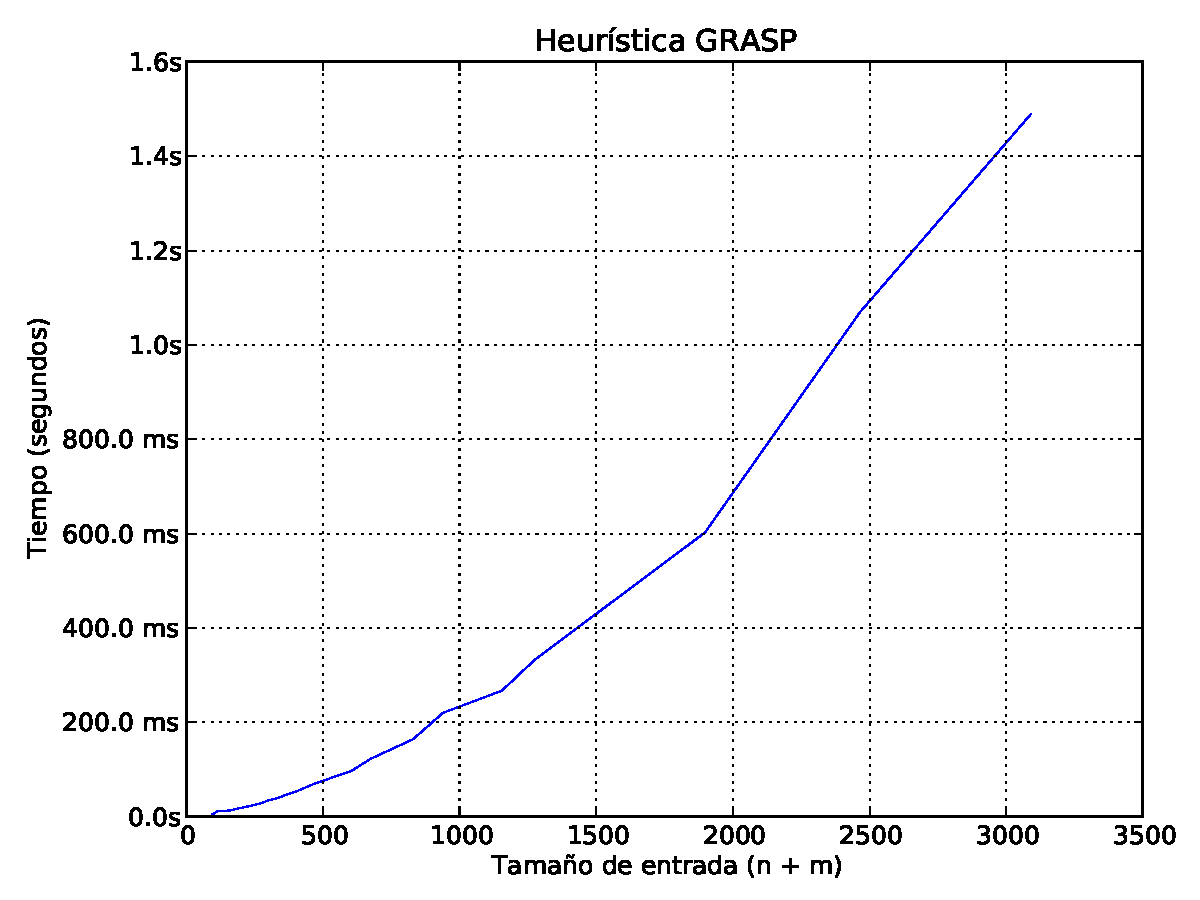
\includegraphics[angle=0, scale=.75]{imagenes/grasp_2014-06-27_19-18-59.pdf}
\label{grafico local}
\end{center}
\end{figure}

No se pareciera estar frente a una polinomio de grado 6, sin embargo, es evidente que tiene mucha más concavidad que la gráfica de la búsqueda
local. Ésto proviene trivialmente del hecho de repetir una cantidad que puede llegar a ser n * log(n) veces la búsqueda local.

Pasamos a experimentar con la calidad de la solución.

\begin{figure}[H]
\begin{center}
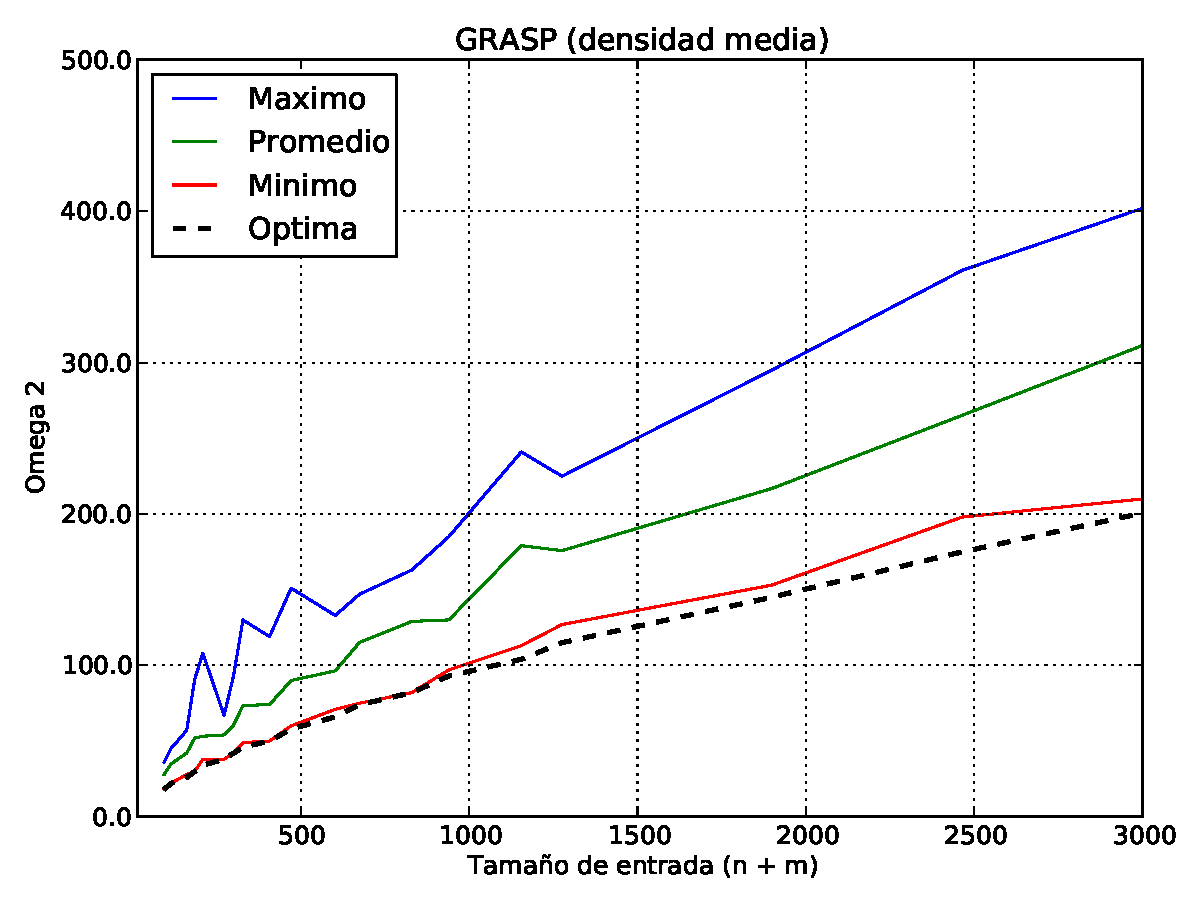
\includegraphics[angle=0, scale=.75]{imagenes/calidad_grasp_2014-06-27_08-58-53.pdf}
\label{grafico local}
\end{center}
\end{figure}

\begin{figure}[H]
\begin{center}
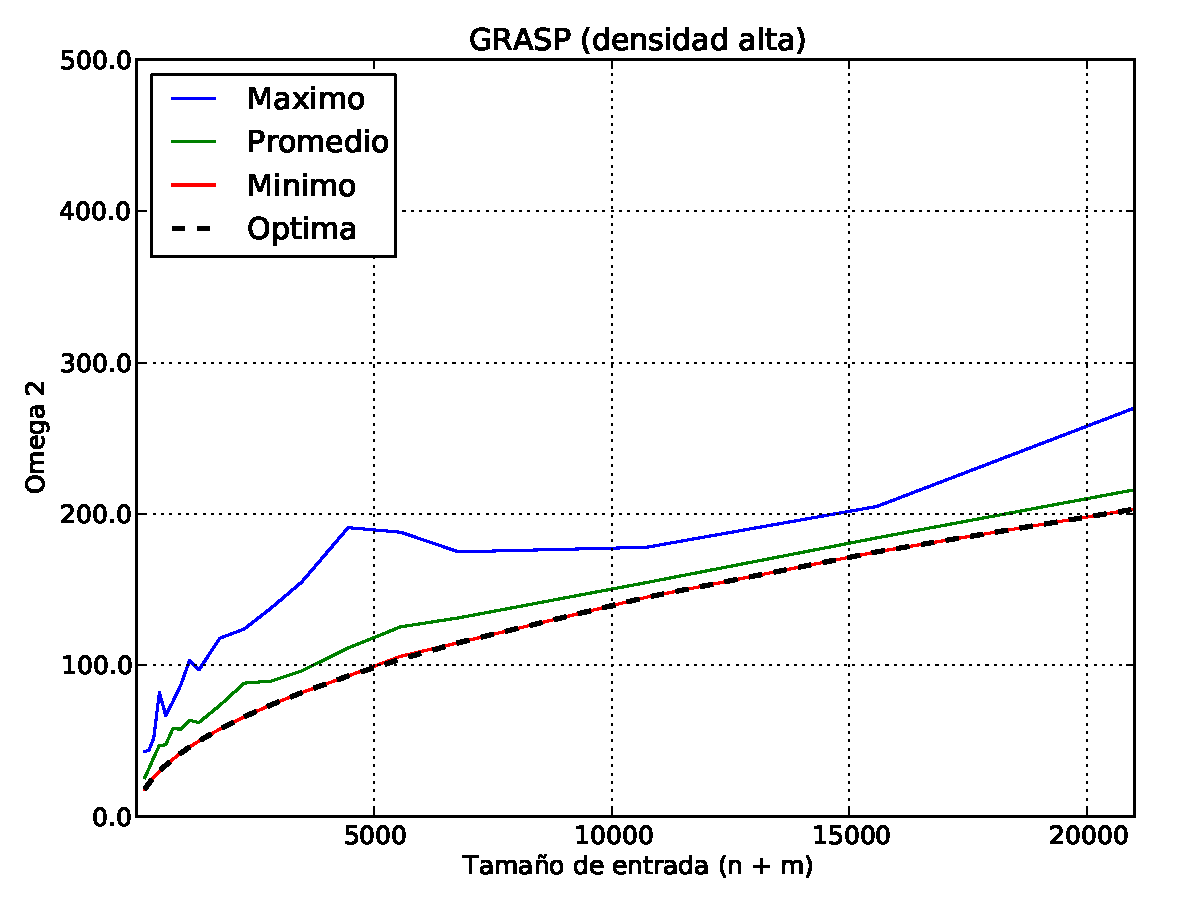
\includegraphics[angle=0, scale=.75]{imagenes/calidad_grasp_2014-06-27_08-54-46.pdf}
\label{grafico local}
\end{center}
\end{figure}

Grata fue la sorpresa al ver a GRASP en acción. Al igual que la búsqueda local, el resultado mínimo de nuestro algoritmo está muy cerca del
óptimo. Pero esta vez hemos logrado reducir la amplitud entre nuestros resultados y de esta forma acercar todo el cuerpo de nuestras soluciones
a la solución óptima.
Los buenos resultados obtenidos se deben a la naturaleza de GRASP, que consiste en iterativamente correr una búsqueda local sobre múltiples
soluciones iniciales generadas con un componente aleatorio. El repetir el experimento disminuye la varianza y garantiza una mejor solución
final.
